\documentclass{article}

\usepackage[left=3cm, right=3cm, top=3cm, bottom=3cm]{geometry}
\usepackage{pdfpages}
\usepackage{cite}
\usepackage{eurosym}
\usepackage[utf8]{inputenc}
\usepackage{graphicx}
\usepackage{amssymb}
\usepackage{amsmath}
\usepackage{array}
\usepackage{graphicx}

\usepackage{breakurl}
\usepackage[breaklinks]{hyperref}

\usepackage{apacite}
\usepackage{gensymb}

\graphicspath{ {./verslag_figuren/} }

\usepackage[numbib]{tocbibind}

\begin{document}

\section{Research}
An important part of a project is research. Without reading through previous experiences or discoveries within the domain of the project, it will be very hard to figure out a solution. Let alone being comfortable enough in the domain to try something drastically new and (hopefully) develop new ideas in the specific branch of the subject. Although image processing is a recent research domain, it is quite popular and already has a lot of foundations to built from. Even Matlab has some predefined functions and libraries to assist the development of image processing software.
However, the goal of this project is to get insight in the programming and working of image processing. To achieve this goal as good as possible, in the end result, there should be little use of predefined functions or libraries. They will only be used if they are completely comprehensible or if they make the code more elegant by doing ordinary operations. 
The next section goes over a few functions which could be used to build on the already existing program described above. All these functions are explained so they can be implemented manually at a later time. It starts by using functions to detect and count the objects, and ends with surrounding the objects with a rectangle, as well as highlighting the edges. An example of these functions can be found in Appendix F.\\

Dit is echt dikke zever

\paragraph{Counting of the objects}\mbox{}\\
The central objective of this paper is counting the amount of objects in a specific rectangular field of view. The general approach to this problem is converting the image to a binary image where black pixels represent the background and white pixels represent the objects. By counting the groups of pixels, it is possible to know how many objects the original image contains. In the image processing toolbox for matlab\cite{Mathworks}, a few functions exist that are very useful for this kind of tasks. One of these functions called bwlabel actually counts group of pixels of at least 8 that are connected. The syntax of this function goes as follows: 
\begin{equation}
[L, num] = bwlabel(BW)
\end{equation}
where BW represents the binary (or black and white) image; num represents the number of objects in the BW image and where L represents a matrix were the first group of pixels are numbered 1, the second group 2 etc. That way it’s easier to get an overview of how many objects there are.

\paragraph{Boundary boxes}\mbox{}\\
The image processing toolbox really simplifies the drawing of boundary boxes. Once a binary image is obtained, the function regionprops \cite{Mathworks} can extract properties about image regions. Where image regions are defined as 8-connected components in an binary image. This means that each image region contains at least 8 interconnected white pixels, since the black pixels are registered as background. The property that's interesting for this part of the project is called 'boundingbox'. This property returns for every image region the smallest rectangle that contains this region. In two dimensions this is a vector with 4 values, the x-coordinate of the upper left corner, the y-coordinate of that corner, the width and the height. The function 
\begin{equation}
rectangle('Position', pos)
\end{equation}
where 'Position' declares the input and where pos is the input obtained from regionprops, can easily display this boundingbox. 

\paragraph{Edge detection}\mbox{}\\
There are a lot of ways to implement edge detection. Edge detection algorithms as described in section 3.2.1 paragraph 4, exist for greyscale images. But if a binary image is available, this becomes much easier. To start, a function called bwboundaries exists in the image processing toolbox \cite{Mathworks}. The syntax of that function goes as follows: 
\begin{equation}
B = bwboundaries (BW)
\end{equation}
where BW represents the input. This is a binary image which only consists out of black and white pixels; and B represents the output, which consist out of a cell array with N elements (number of image regions in the binary image), all these elements contain a list of the boundary pixels. Which in turn are fairly easy to draw. They can be inserted in the matrix of the image by replacing values, this is done by looping through the cell arrays. The advantage of this method is that the image can actually be printed. When they are drawn on top of the image with a function like visboundaries, the actual values of the pixels stay unchanged, but it different figures arise. One with the image and another on top of it with the edges. 
The function bwboundaries implements the Moore-Neighbor tracing algorithm \cite{Moore_Neighborhood}. The algorithm loops through the entire matrix until it finds a white pixel (a pixel that belongs to an image region). This pixel is defined as the start pixel. Once it finds a start pixel it searches for the next connected white pixel. This means another white pixel in one of the eight regions around the start. The algorithm does this by examining the pixels in a clockwise direction. Once it finds a new white pixel, this pixel is added to the sequence B and becomes our new start pixel. This process keeps on running until the algorithm visits the first start pixel for a second time. The only problem with this algorithm is that sometimes the first start pixel is visited for a second time before all of the outline is visited. This is illustrated in Fig.~\ref{fig:Moore_Neighbor}).

\begin{figure}[h]
	\center
  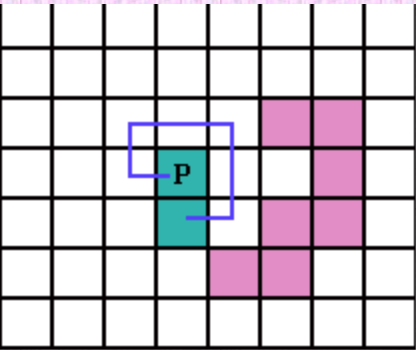
\includegraphics[width=0.3\linewidth]{Moore_Neighbor.png}
  \caption{Problem with stopping criteria Moore-Neighbor tracing algorithm.\cite{Moore_Neighborhood}}
  \label{fig:Moore_Neighbor}
\end{figure}

\noindent This problem is resolved with the Jacob's stopping criterion. Which states that the algorithm can stop once the first start pixel is visited from the same direction as it initially was entered. This leaves four possibilities that need to be checked, from below, from the left, from above or from the right. With this additional criteria, every pixel at the edge of a connected region is visited. 
To find the edges of all the interconnected image regions this process is repeated until every pixel of the image matrix has been checked. 

\end{document}